\chapter{龙芯新增浮点指令}

\newcommand{\fmt}{{\sl fmt}}
\newcommand{\ps}{{\sl ps}}

\section{单精度对指令}

\begin{table}[htbp]
  \centering
  \begin{tabular}{|>{\centering}p{2cm}|>{\raggedleft}p{2.5cm}@{.}>{\raggedright}p{1.5cm}|
                  |>{\centering}p{2cm}|>{\raggedleft}p{2.5cm}@{.}>{\raggedright}p{1.5cm}|} \hline
    OP & \multicolumn{2}{c||}{OP(\fmt = 22)} &
    OP & \multicolumn{2}{c| }{OP(\fmt = 22)} \tabularnewline \hhline
    ADD         & ADD         & \ps & C.{\sl ult}  & C.{\sl ult}  & \ps \tabularnewline
    MADD        & MADD        & \ps & C.{\sl ole}  & C.{\sl ole}  & \ps \tabularnewline
    MSUB        & MSUB        & \ps & C.{\sl ule}  & C.{\sl ule}  & \ps \tabularnewline
    NMADD       & NMADD       & \ps & C.{\sl sf}   & C.{\sl sf}   & \ps \tabularnewline
    NMSUB       & NMSUB       & \ps & C.{\sl ngle} & C.{\sl ngle} & \ps \tabularnewline
    SUB         & SUB         & \ps & C.{\sl seq}  & C.{\sl seq}  & \ps \tabularnewline
    NEG         & NEG         & \ps & C.{\sl ugl}  & C.{\sl ugl}  & \ps \tabularnewline
    ABS         & ABS         & \ps & C.{\sl lt}   & C.{\sl lt}   & \ps \tabularnewline
    C.{\sl f}   & C.{\sl f}   & \ps & C.{\sl nge}  & C.{\sl nge}  & \ps \tabularnewline
    C.{\sl un}  & C.{\sl un}  & \ps & C.{\sl le}   & C.{\sl le}   & \ps \tabularnewline
    C.{\sl eq}  & C.{\sl eq}  & \ps & C.{\sl ngt}  & C.{\sl ngt}  & \ps \tabularnewline
    C.{\sl ueq} & C.{\sl ueq} & \ps & MUL          & MUL          & \ps \tabularnewline
    C.{\sl olt} & C.{\sl olt} & \ps & MOV          & MOV          & \ps \tabularnewline \hline
  \end{tabular}
  \caption{龙芯单精度对指令}
  \label{tab:paired-single}
\end{table}


\section{新增浮点指令}

\subsection{MADD.\fmt (浮点乘加)}

\begin{instructionblk}
  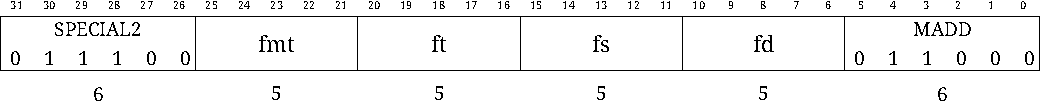
\includegraphics{ins-MADD} \\
  \instructionbody
  {MADD.S fd, fs, ft \newline
  MADD.D fd, fs, ft}
  {浮点值的先乘后加。}
  {{\tt fd $\leftarrow$ (fs * ft) + fd;} \fldnewline
  先将浮点寄存器ft中的值乘以浮点寄存器fs中的值,得到一个乘积。再把这个乘积加
  上浮点寄存器fd中的值,得到运算结果。这个运算指令结果有很高的精度,发生进位时
  的处理方式是按照FCSR的当前进位模式,结果保存进fd中。操作数和运算结果都是\fmt 
  格式。}
  {vfd $\leftarrow$ ValueFPR(fd, fmt); \newline
  vfs $\leftarrow$ ValueFPR(fs, fmt); \newline
  vft $\leftarrow$ ValueFPR(ft, fmt); \newline
  StoreFPR(fd, fmt, vfd + vfs * vft);}
  {不可用协处理器例外 \newline
  保留指令例外 \newline
  浮点:\newline
  \begin{tabular}{@{\hspace{1cm}}p{3cm}p{3cm}p{3cm}}
    不精确例外 & 未实现操作例外 & 无效操作例外 \tabularnewline
    上溢例外 & 下溢例外
  \end{tabular}}
\end{instructionblk}

\subsection{MSUB.\fmt (浮点乘减)}

\begin{instructionblk}
  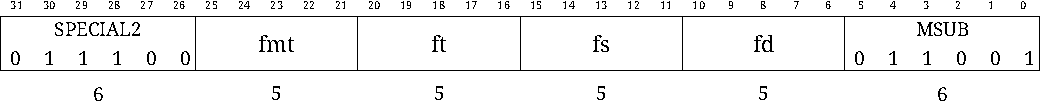
\includegraphics{ins-MSUB} \\
  \instructionbody
  {MSUB.S fd, fs, ft \newline
  MSUB.D fd, fs, ft}
  {浮点值的先乘后减。}
  {{\tt fd $\leftarrow$ (fs * ft) - fd;} \fldnewline
  先将浮点寄存器ft中的值乘以浮点寄存器fs中的值,得到一个乘积。再把这个乘积减
  去浮点寄存器fd中的值,得到运算结果。这个运算指令结果有很高的精度,发生进位时
  的处理方式是按照FCSR的当前进位模式,结果保存进fd中。操作数和运算结果都是\fmt 
  格式。}
  {vfd $\leftarrow$ ValueFPR(fd, fmt); \newline
  vfs $\leftarrow$ ValueFPR(fs, fmt);  \newline
  vft $\leftarrow$ ValueFPR(ft, fmt);  \newline
  StoreFPR(fd, fmt, (vfs * vft) - vfd);}
  {不可用协处理器例外 \newline
  保留指令例外 \newline
  浮点:\newline
  \begin{tabular}{@{\hspace{1cm}}p{3cm}p{3cm}p{3cm}}
    不精确例外 & 未实现操作例外 & 无效操作例外 \tabularnewline
    上溢例外 & 下溢例外
  \end{tabular}}
\end{instructionblk}


\subsection{NMADD.\fmt (浮点乘加取负)}

\begin{instructionblk}
  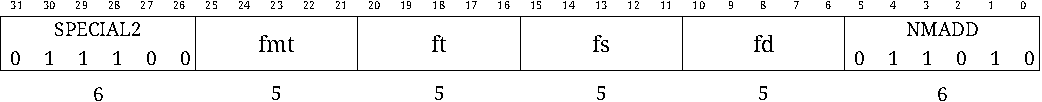
\includegraphics{ins-NMADD} \\
  \instructionbody
  {NMADD.S fd, fs, ft \newline
  NMADD.D fd, fs, ft}
  {对先乘后加的结果取负。}
  {{\tt fd $\leftarrow$ -((fs * ft) + fd);} \fldnewline
  先将浮点寄存器ft中的值乘以浮点寄存器fs中的值,得到一个乘积。再把这个乘积加
  上浮点寄存器fd中的值,再把和值取负得到运算结果。这个运算指令结果有很高的精度,
  发生进位时的处理方式是按照FCSR的当前进位模式,结果保存进fd中。操作数和运算结
  果都是\fmt 格式。}
  {vfd $\leftarrow$ ValueFPR(fd, fmt); \newline
  vfs $\leftarrow$ ValueFPR(fs, fmt);  \newline
  vft $\leftarrow$ ValueFPR(ft, fmt);  \newline
  StoreFPR(fd, fmt, -((vfs * vft) + vfd);}
  {不可用协处理器例外 \newline
  保留指令例外 \newline
  浮点:\newline
  \begin{tabular}{@{\hspace{1cm}}p{3cm}p{3cm}p{3cm}}
    不精确例外 & 未实现操作例外 & 无效操作例外 \tabularnewline
    上溢例外 & 下溢例外
  \end{tabular}}
\end{instructionblk}

\subsection{NMSUB.\fmt (浮点乘减取负)}

\begin{instructionblk}
  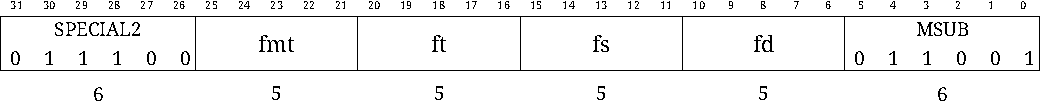
\includegraphics{ins-MSUB} \\
  \instructionbody
  {NMSUB.S fd, fs, ft \narrownewline NMSUB.D fd, fs, ft}
  {对先乘后减的结果取负。}
  {{\tt fd $\leftarrow$ -((fs * ft) - fd);} \fldnewline
  先将浮点寄存器ft中的值乘以浮点寄存器fs中的值,得到一个乘积。再把这个乘积减
  去浮点寄存器fd中的值,再把差值取负得到运算结果。这个运算指令结果有很高的精度,
  发生进位时的处理方式是按照FCSR的当前进位模式,结果保存进fd中。操作数和运算结
  果都是\fmt 格式。}
  {vfd $\leftarrow$ ValueFPR(fd, fmt); \newline
  vfs $\leftarrow$ ValueFPR(fs, fmt); \newline
  vft $\leftarrow$ ValueFPR(ft, fmt); \newline
  StoreFPR(fd, fmt, -((vfs * vft) - vfd));}
  {不可用协处理器例外 \newline
  保留指令例外 \newline
  浮点:\newline
  \begin{tabular}{@{\hspace{1cm}}p{3cm}p{3cm}p{3cm}}
    不精确例外 & 未实现操作例外 & 无效操作例外 \tabularnewline
    上溢例外 & 下溢例外
  \end{tabular}}
\end{instructionblk}

